\section{Progress}
\label{sec:Progress}


\begin{figure}[t!]
\centering
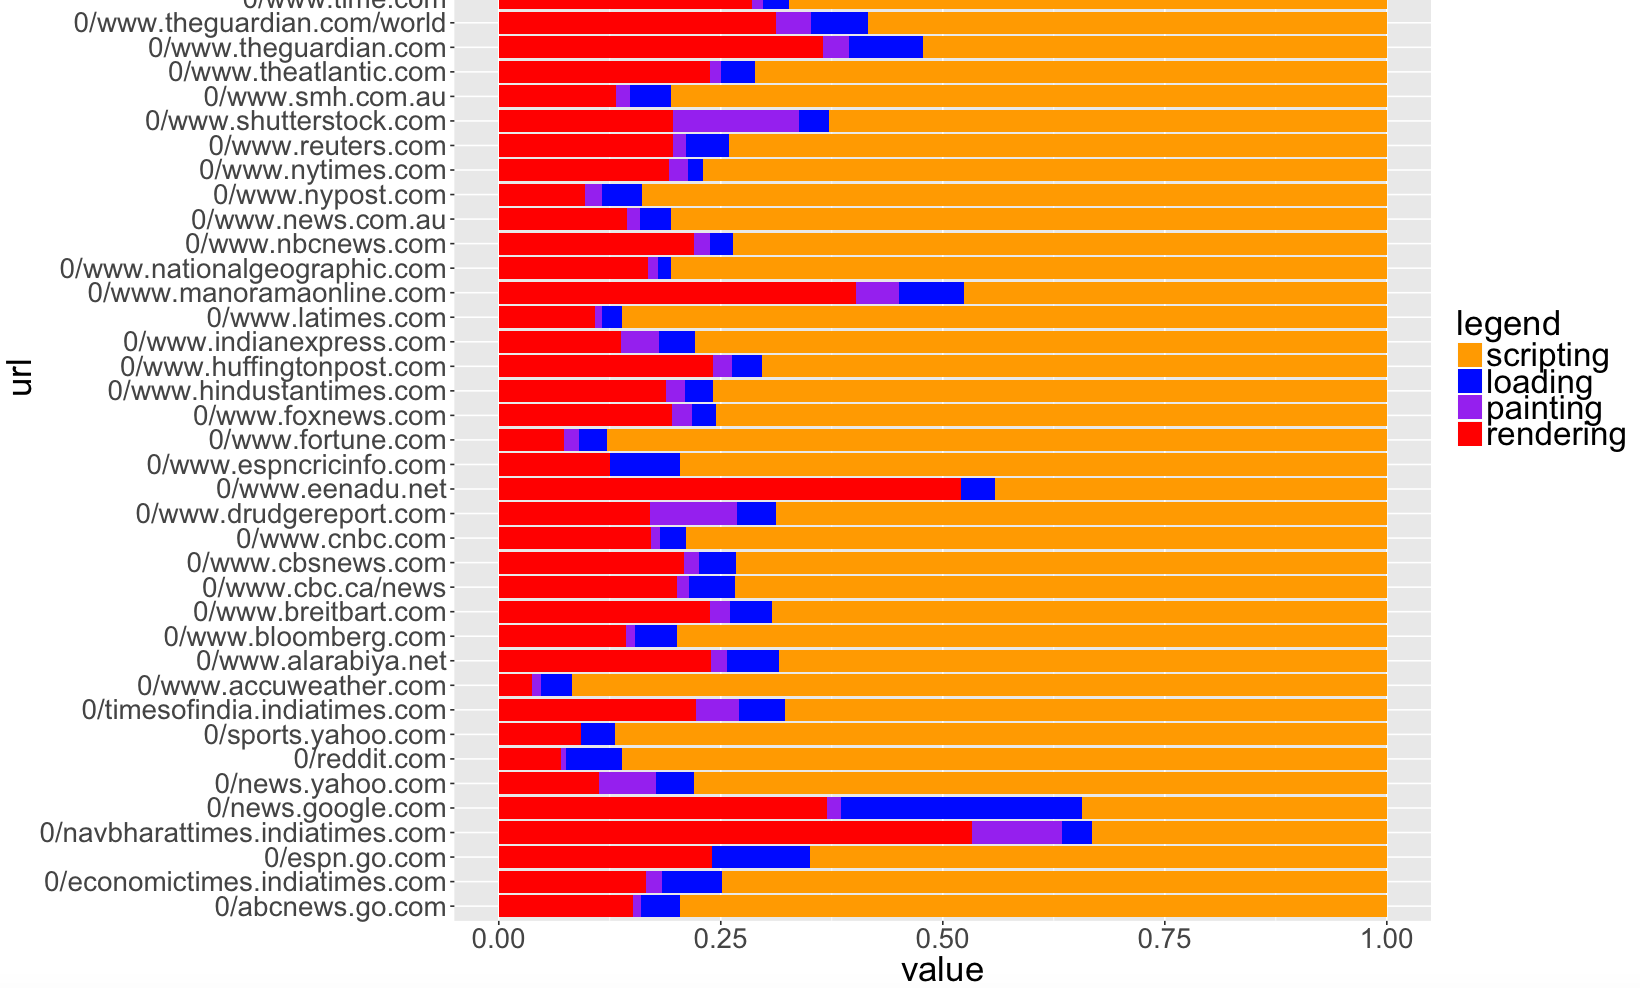
\includegraphics[width=0.99\columnwidth, scale=2.0]{figs/comp_1.png}
\tightcaption{Breakdown of computation on pixel 2}
\label{fig:act_p2}
\end{figure}

As a preeliminary step in research, we first established a corpus of the top
75 news and sports websites on which we woudl run most of our experiments
in order to cater to the most popular and compute intensive websites. 
These websites are taken from the Alexa top website list.
We ran all our experiments on  Google Pixel 2. We used chrome v 61 to run all  our experiments
both on the mobile device. We leveraged chrome developer tools in order
to capture the runtime traces both for network and compute. We then analysed these runtime
traces to draw insight into the critical path of the website, the total time being spent on the 
compute vs the total time being spent on the network, and most importantly the finer
level breakdown of the computation time to understand the true nature of computation on mobile
devices. 

We categorised computation time into four categorires, scripting, loading, rendering and
painting. Scripting is the total time being spent on
compiling javascript, evaluating and executing it. Loading is the parsing of html and css, which happens 
immediately after the payload for the network requests are received by the browser. Loading essentially
takes these payload objects and parses them and converts them to a DOM tree. Once the DOM tree is built,
the rendering engine kicks in which starts to convert this DOM tree into a render tree, which contains the
exact coordinates and the shape of each of the DOM node. This is what rendering time comprises of. 
Painting time is the time taken to process the render tree, and actually convert
each pixel into a bitmap.
Figure 3 shows the computation break down for these first level of categories
for Google pixel 2. We further break down this time into the most finest level events
which are returned by Google Chrome's trace and then group them by their event name.

\begin{figure}[t!]
\centering
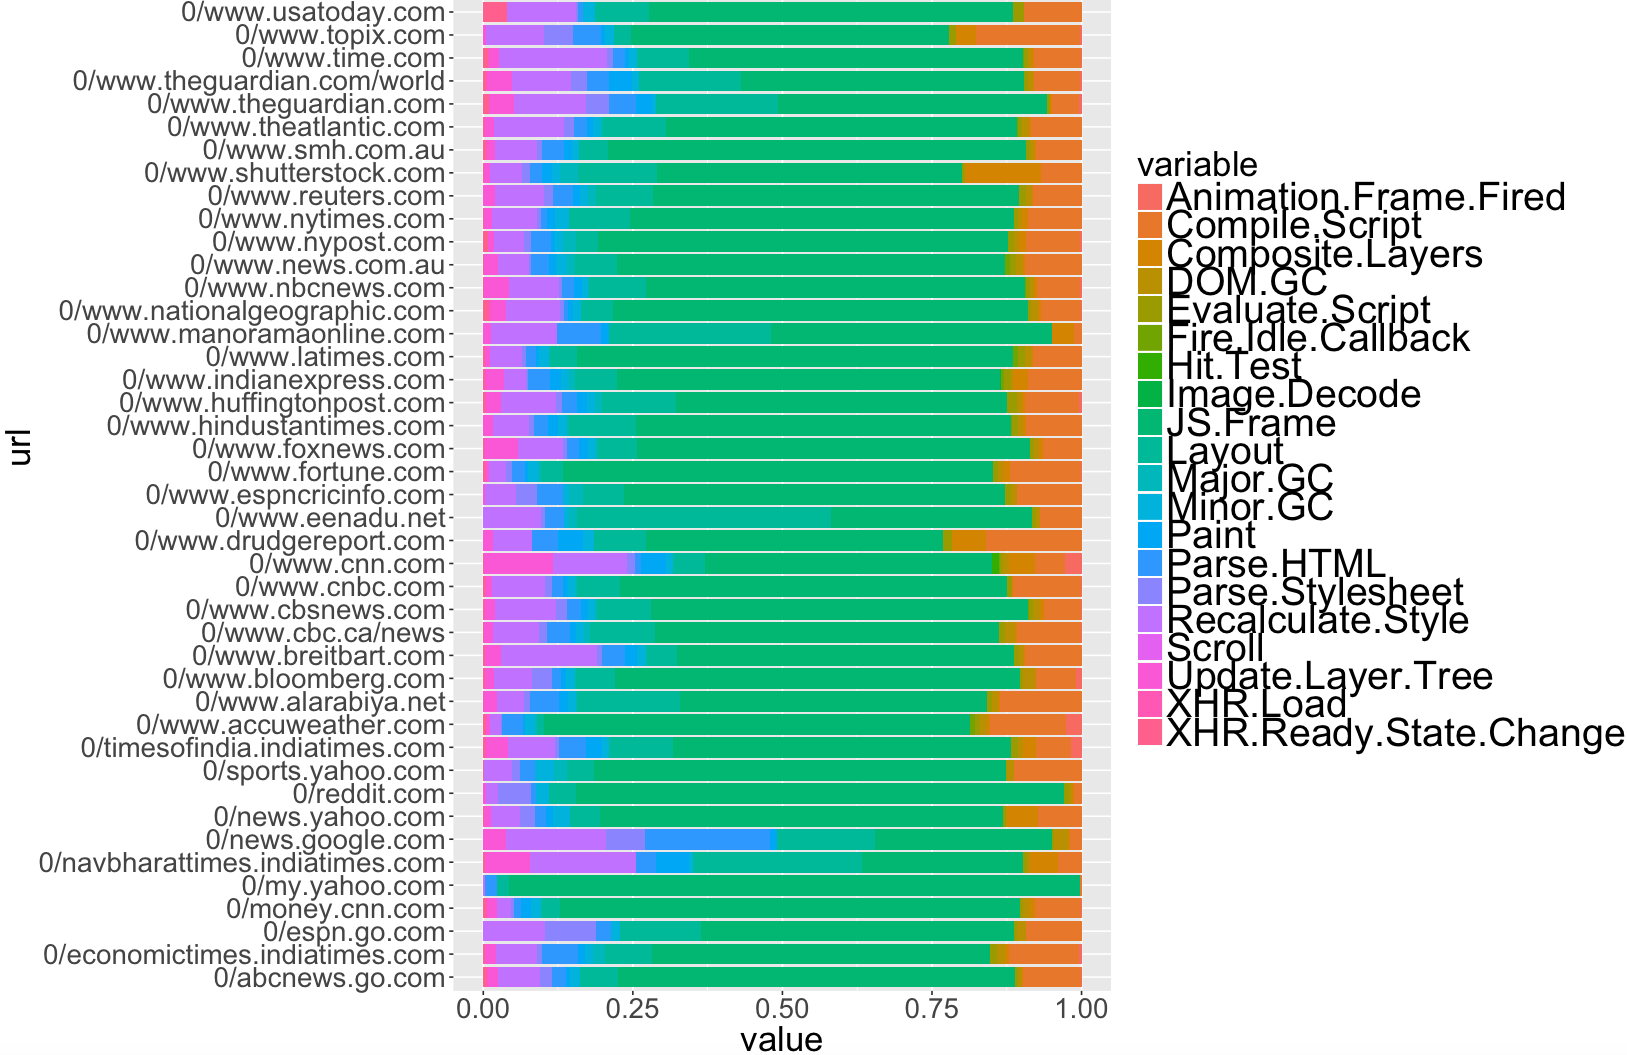
\includegraphics[width=0.9\columnwidth]{figs/comp_2.png}
\tightcaption{Breakdown of computation into finer events on pixel 2}
\label{fig:cat_p2}
\end{figure}


These results are extremely coherent with our design of implementing a javsvcript chrome
caching mechanism and show the possibility of a large improvement in the total page
load due to the high percentage share of execution time as seen in Figure 4. 

\begin{figure}[t]
\centering
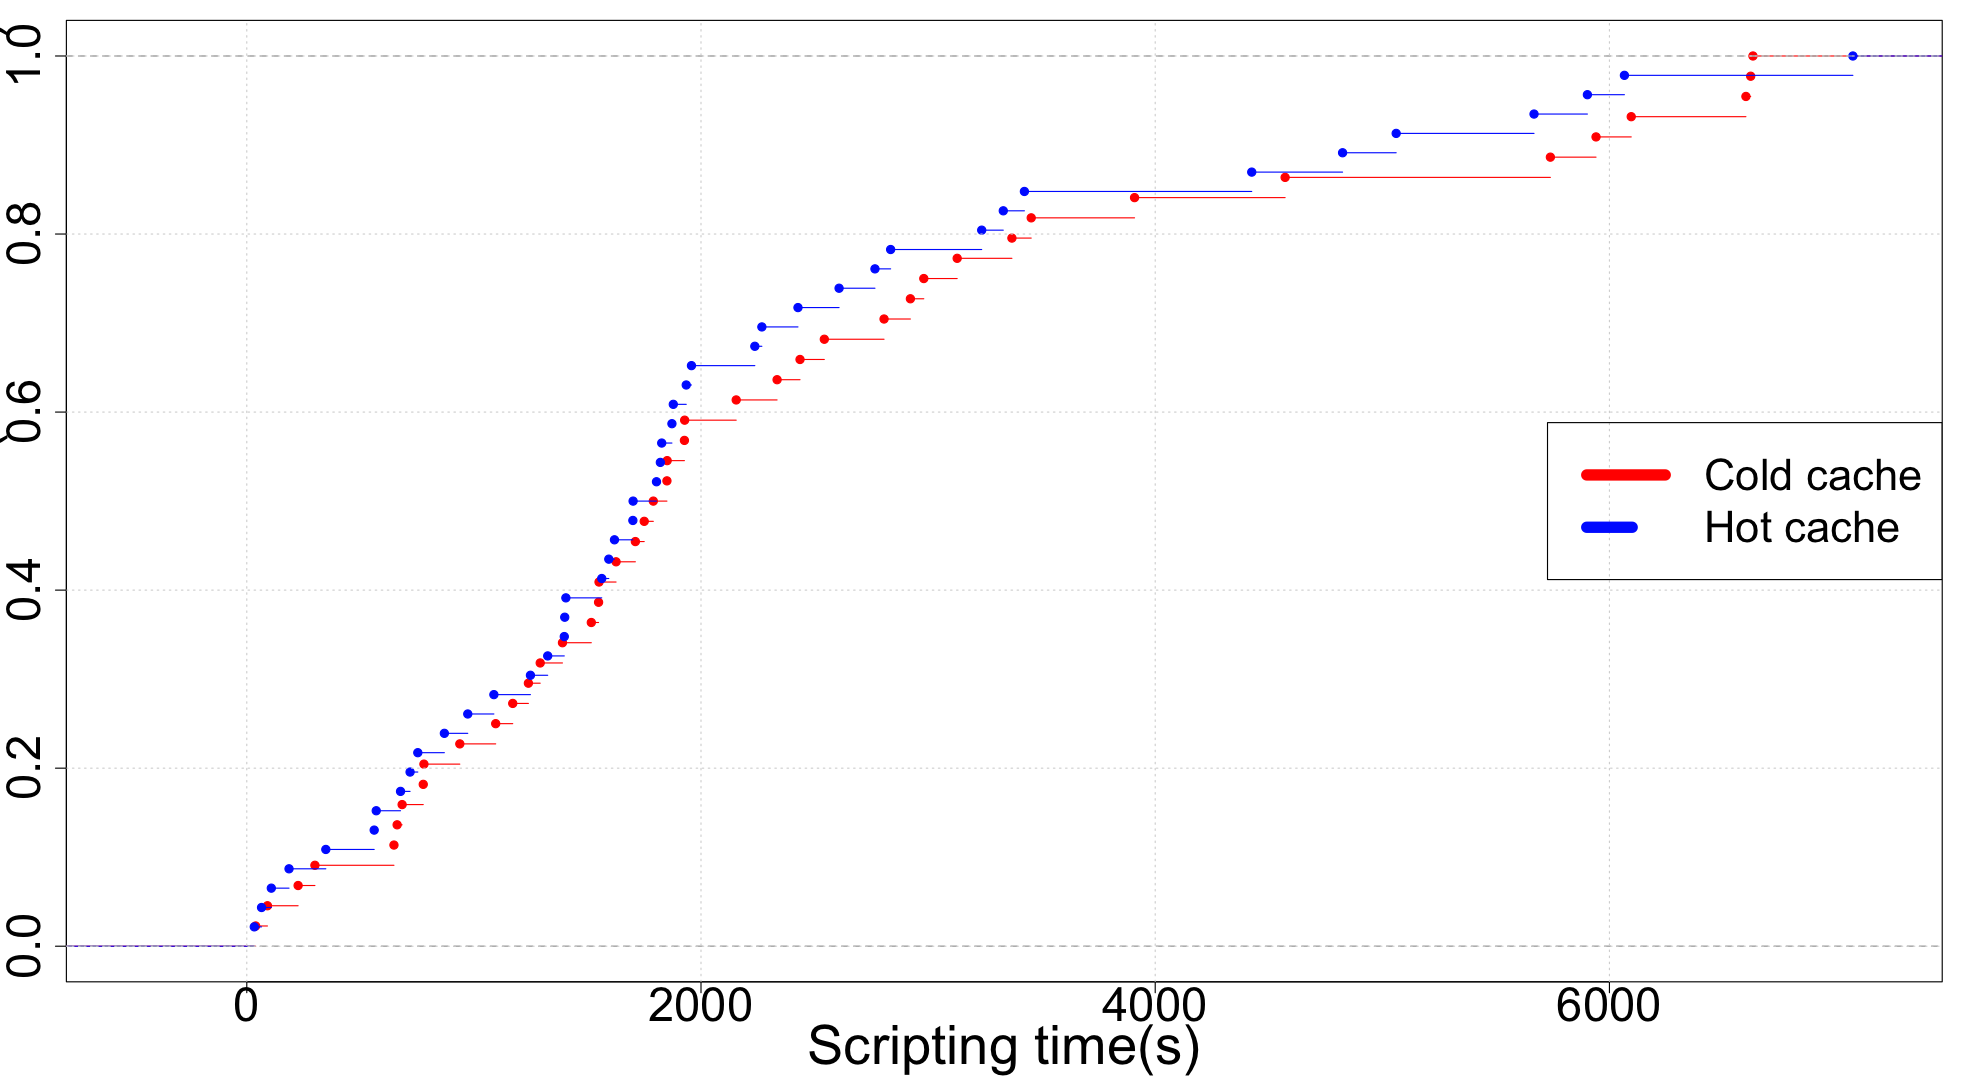
\includegraphics[width=0.9\columnwidth]{figs/chrome_script.png}
\tightcaption{CDF of scripting time with and without chrome's optimisations}
\label{fig:scripting_p2}
\end{figure}

Recently Chrome in their 2017 dev summit talked about the various optimisation techniques
they have employed in the latest Chrome browser to improve the total page load time.
We did a comparison of the total page load time with and without chrome's optimisation to see
the improvements. In order to do this, we captured the trace from Alexa's top 75 
news and sports website once with a fresh cache, ie cold cache and then subsequently with a hot
cache which contains all of Chrome's optimisation including it's compiler and parser cache. 
As we can see from figure 7, there has been a significant reduction in the overall compilation
time, with about 100ms reduction in median compile time. This is primarily due to the introduction of compiler and parser cache. 
The line corresponding to Cold cache refers to fresh load of all the websites,
whereas the line corresponding to the Hot cache refers to the subsequent load
which makes use of the Chrome's caching framework. 
This is also reflected partially in the overall scripting time
as shown in Figure 5. Note that scripting time is the sum of compilation, execution and other
minor javascript events in the execution pipeline like garbage collection. 
However the interesting thing to note, is that despite all these optimisations,
we observe almost neglible improvement in the median execution time of javascripts, as
shown in Figure 6. This serves as a huge motivation for the vaste potential in
improvement of the overall page load time, by optimising the javascript execution
time.

\begin{figure}[t]
\centering
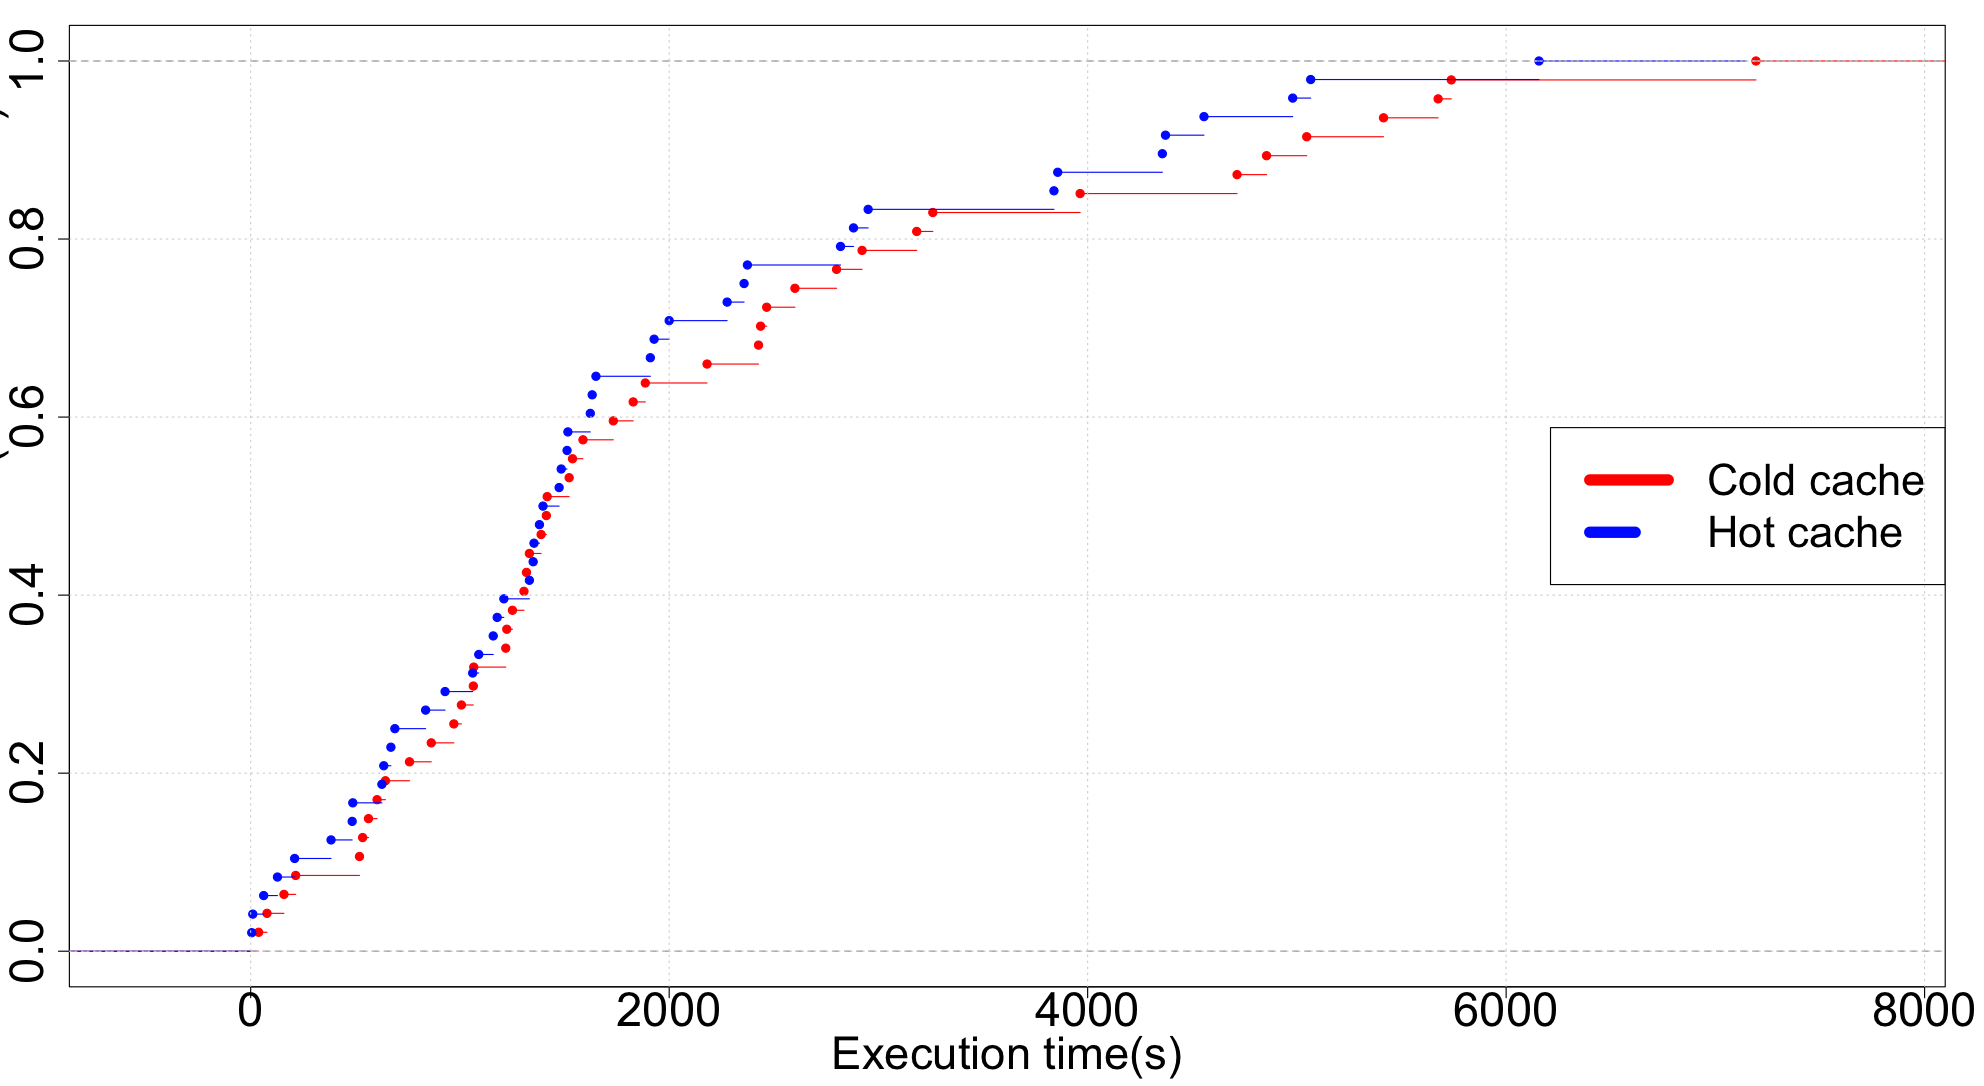
\includegraphics[width=0.9\columnwidth]{figs/chrome_exec.png}
\tightcaption{CDF of total execution time with and without chrome's optimisations}
\label{fig:compile_p2}
\end{figure}

\begin{figure}[t]
\centering
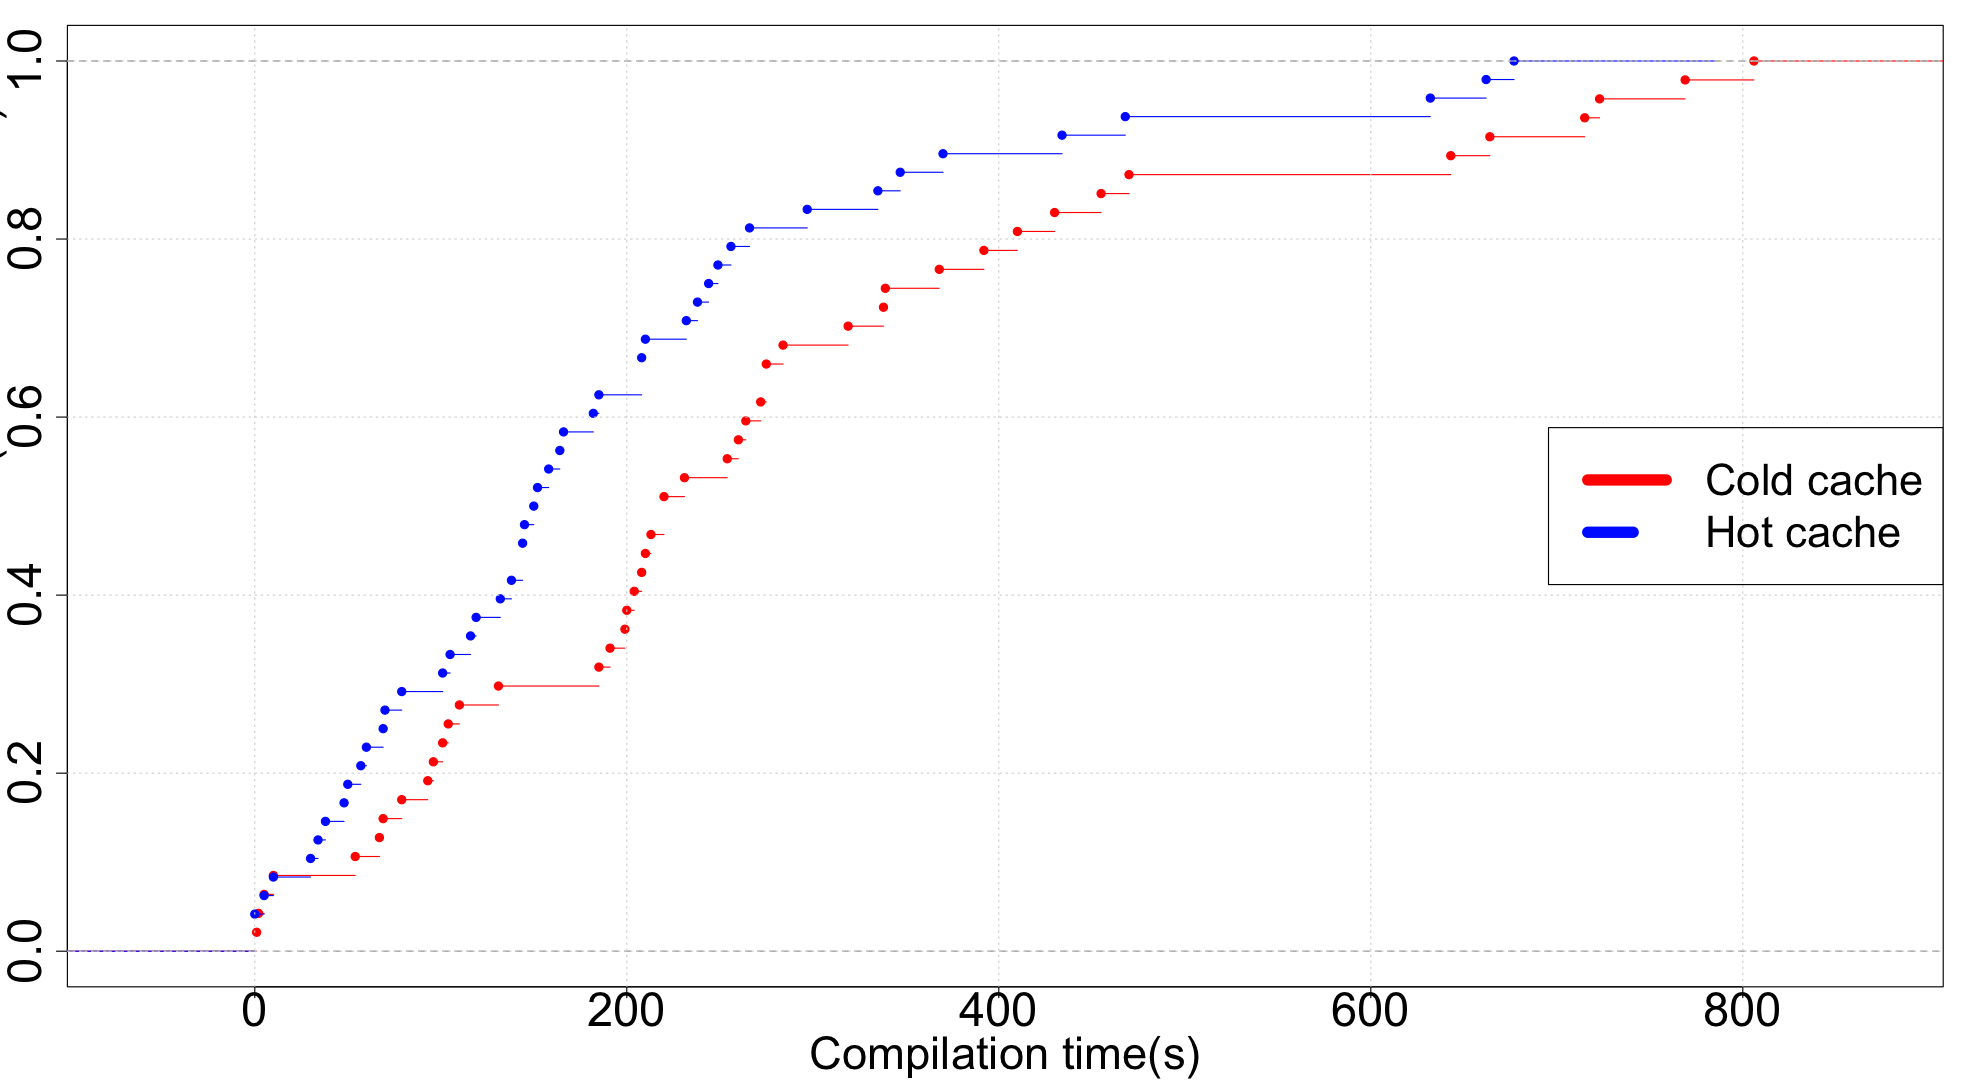
\includegraphics[width=0.9\columnwidth]{figs/chrome_compile.png}
\tightcaption{CDF of compilation time with and without chrome's optimisations}
\label{fig:compile_p2}
\end{figure}

